\documentclass[11pt,a4paper]{article}
\usepackage[utf8]{inputenc}
\usepackage[T1]{fontenc}
\usepackage{graphicx}
\usepackage{booktabs}
\usepackage{geometry}
\usepackage{hyperref}
\usepackage{float}
\usepackage{titlesec}
\usepackage{amsmath}
\usepackage{parskip}

\geometry{margin=1in}

\title{\textbf{Predicting Fast-Growing Firms: Summary Report}}
\author{Data Analysis 3 - Assignment 2 \\ Submitted by: Balint Decsi (ID: 2506626), Zariza Chowdhury (ID: 2500086) \\ \url{https://github.com/zarizachow/Data-Analysis-3/tree/main}}
\date{February 2026}

\begin{document}

\maketitle

\section*{Executive Summary}

This report outlines the development and evaluation of predictive models designed to identify fast-growing firms using the Bisnode dataset. Our analysis defines "fast growth" as firms achieving the top 10\% of sales growth year-over-year (2013 vs. 2012). 

\textbf{Key Decision:} We recommend deploying the \textbf{Random Forest} model. It significantly outperforms traditional logistic regression benchmarks in identifying high-potential firms, reducing the expected business loss by approximately 20\% under our specified cost structure.

\section*{Target Definition \& Business Problem}

We define a fast-growing firm as one in the top decile (top 10\%) of log sales growth from 2012 to 2013. The distribution of firm growth is shown below.

\begin{figure}[H]
    \centering
    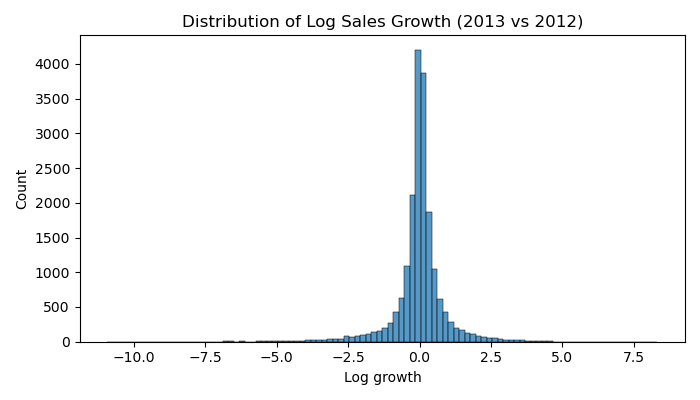
\includegraphics[width=0.7\textwidth]{Assignment-2/Output/Plots/growth_log_distribution.png}
    \caption{Distribution of Log Sales Growth (2012-2013)}
\end{figure}

\begin{itemize}
    \item \textbf{Why this target?} Focusing on the top decile isolates the truly high-performers from steady-state firms. A one-year horizon (2012-2013) was chosen over a two-year horizon (2012-2014) to minimize \textbf{mean reversion effects}, where high growth naturally decays over longer periods, and to avoid \textbf{survivorship bias} that would exclude riskier, high-volatility firms from the sample. This provides a more immediate and actionable signal for investment.
    \item \textbf{Business Objective:} The goal is to invest in or target these firms early. Missing a fast grower (False Negative) is considered significantly more costly than investigating a false lead (False Positive).
    \item \textbf{Loss Function:} We assigned a cost ratio where the cost of a False Negative (FN) is \textbf{4 times} that of a False Positive (FP).
    \[ \text{Loss} = 1 \times \text{FP} + 4 \times \text{FN} \]
\end{itemize}

\section*{Model Performance Comparison}

We evaluated three models: Logistic Regression (L2 regularization), LASSO (L1 regularization), and Random Forest. The non-linear nature of growth drivers, such as firm age, is a key reason for using flexible models like Random Forest.

\begin{figure}[H]
    \centering
    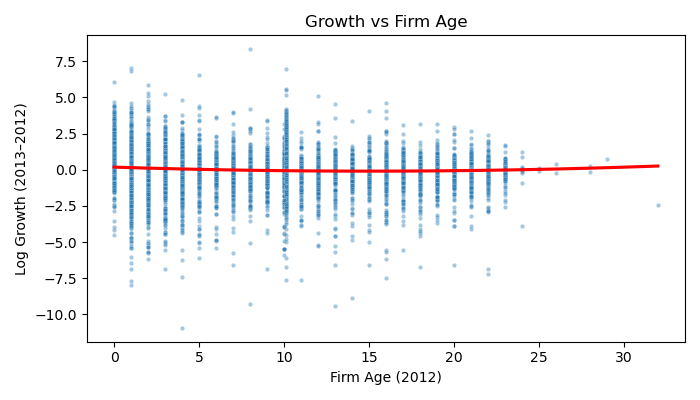
\includegraphics[width=0.7\textwidth]{Assignment-2/Output/Plots/growth_vs_age.png}
    \caption{Growth vs. Firm Age: Younger firms show higher but more volatile growth.}
\end{figure}

\begin{table}[H]
    \centering
    \caption{Model Performance (Probability Prediction)}
    \begin{tabular}{lccc}
        \toprule
        \textbf{Model} & \textbf{ROC-AUC} & \textbf{Avg Precision} & \textbf{Brier Score} \\
        \midrule
        \textbf{Random Forest} & \textbf{0.828} & \textbf{0.460} & \textbf{0.078} \\
        Logit (LASSO) & 0.753 & 0.269 & 0.121 \\
        Logit (L2) & 0.753 & 0.269 & 0.121 \\
        \bottomrule
    \end{tabular}
\end{table}

The \textbf{Random Forest} model dominates the linear models. An AUC of 0.828 indicates strong discriminatory power. Notably, the Average Precision (0.460) is nearly double that of the Logit models, meaning that when the model predicts a firm is fast-growing, it is much more likely to be correct.

\section*{Decision Threshold \& Expected Loss}

To minimize business loss (prioritizing the capture of fast growers), we optimized the classification threshold for each model.

\begin{table}[H]
    \centering
    \caption{Optimal Classification Performance (Lower is Better)}
    \begin{tabular}{lcc}
        \toprule
        \textbf{Model} & \textbf{Avg Expected Loss} & \textbf{Optimal Threshold} \\
        \midrule
        \textbf{Random Forest} & \textbf{0.255} & \textbf{0.150} \\
        Logit (L2) & 0.316 & 0.446 \\
        \bottomrule
    \end{tabular}
\end{table}

The Random Forest model yields an average expected loss of \textbf{0.255}, which is substantially lower than the Logit model's 0.316. The optimal probability threshold is approximately \textbf{15\%}. This means if the model assigns a probability of fast growth greater than 15\%, we should classify the firm as a target. This low threshold reflects our preference to avoid missing opportunities (high cost of False Negatives).

\section*{Industry Analysis}

We validated the model across two key sectors: \textbf{Manufacturing} and \textbf{Services} (Repair, Accommodation, Food).

\begin{itemize}
    \item \textbf{Manufacturing:} AUC = 0.817 | Expected Loss = 0.239
    \item \textbf{Services:} AUC = 0.838 | Expected Loss = 0.257
\end{itemize}

The model is robust across sectors, performing slightly better in the Services sector in terms of ranking (AUC) but incurring slightly higher loss due to sector-specific difficulty. It is safe to deploy the model in both domains.

\section*{Conclusion \& Recommendation}

We recommend implementing the \textbf{Random Forest} model for targeting fast-growing firms. 
\begin{enumerate}
    \item \textbf{High Accuracy:} It captures non-linear relationships (e.g., between age/size and growth) that linear models miss.
    \item \textbf{Cost Effective:} It minimizes the weighted business loss effectively.
    \item \textbf{Actionable:} Using a probability threshold of 15\%, the sales/investment team can create a prioritized list of high-potential targets.
\end{enumerate}

\end{document}
